%-*- program: xelatex -*-        
%-*- program: biber -*-`        
%-*- program: xelatex -*-
\documentclass[12pt]{article}
\usepackage{amsmath,textcomp,amssymb,geometry,graphicx,enumerate,upquote,color}
\usepackage{hyperref}
\usepackage{float}
\usepackage{tikz}
\usepackage{array}
\usepackage{amsfonts}
\def\Session{Fall 2015}
\usepackage[english]{babel}
\title{Exploratory Analysis of Various Assets}
\author{Boying Gong, Xinyue Zhou}
\newenvironment{qparts}{\begin{enumerate}[{(}a{)}]}{\end{enumerate}}
\def\endproofmark{$\Box$}
\newenvironment{proof}{\par{\bf Proof}:}{\endproofmark\smallskip}
\begin{document}
\maketitle

\section{Description}
\subsection{US Equity}

\begin{itemize}
\item AGG: iShares Core US Aggregate Bond\\
Date ranges: 2003-09-29 to 2015-12-31\\
Components: US Treasuries (37.7\%);
US Agencies (2.5\%); US Municipals (0.8\%);
Corporates (24.2\%); Non-Corporate Credit (4.4\%); Mortgage-Backed Securities (MBS) (28.4\%); Commercial Mortgage-Backed Securities (CMBS) (1.7\%); Adjusted Rate Mortgages (ARMs) (0.2\%)
\\
Description: AGG provides access to 4,000+ bonds and offers exposure to 7 unique sectors as represented in the broad U.S. bond market. \footnote{https://www.ishares.com/us/literature/product-brief/ishares-core-us-aggregate-bond-etf-product-brief-en-us.pdf}
\item HYG: iShares iBoxx \$ High Yield Corporate Bd\\
Date ranges: 2007-04-12 to 2015-12-31\\
Components:The sector breakdown data  shows that four sectors occupied more than 10\% high yield bond, those are: Communications(25.8\%), Consumer Non-cyclical(14.2\%), Energy(11.4\%), Technology(10.7\%)\footnote{https://www.ishares.com/us/literature/product-brief/ishares-iboxx-high-yield-corporate-bond-etf-profile-en-us.pdf}\\
Description: The iShares iBoxx \$ High Yield Corporate Bond ETF seeks to track the investment results of an index composed of U.S. dollar-denominated, high yield corporate bonds. \footnote{https://www.ishares.com/us/products/239565/ishares-iboxx-high-yield-corporate-bond-etf}

\item TIP: iShares TIPS Bond\\
Date ranges: 2003-12-08 to 2015-12-31\\
Components: government bonds. \\
Description: Seeks to track the investment results of an index composed of inflation-protected U.S. Treasury bonds.\footnote{https://www.ishares.com/us/literature/fact-sheet/tip-ishares-tips-bond-etf-fund-fact-sheet-en-us.pdf}
\end{itemize}

\subsection{Index}

\begin{itemize}
\item BCOM: Bloomberg Commodity Index\\
Date ranges: 1991-01-03 to 2015-12-31\\
Description: Bloomberg Commodity Index (BCOM) is calculated on an excess return basis and reflects commodity futures price movements. The index rebalances annually weighted 2/3 by trading volume and 1/3 by world production and weight-caps are applied at the commodity, sector and group level for diversification. Roll period typically occurs from 6th-10th business day based on the roll schedule.\footnote{http://www.bloomberg.com/quote/BCOM:IND}
% \item BUHY: Bloomberg USD High Yield Corporate Bond Index\\
% Date ranges: 2010-01-04 to 2015-12-31 \\
% Description: The Bloomberg USD High Yield Corporate Bond Index is a rules-based, market-value weighted index engineered to measure publicly issued non-investment grade USD fixed-rate, taxable, corporate bonds. To be included in the index a security must have a minimum par amount of 250MM.\footnote{http://www.bloomberg.com/quote/BUHY:IND}
\item G0O1: 3-Month U.S. Treasury Bill Index\\
Date ranges: 1992-04-01 to 2015-12-31 \\
Description: The US 3-Month Treasury Bill Index is comprised of a single issue purchased at the beginning of the
month and held for a full month. At the end of the month that issue is sold and rolled into a newly selected issue. The
issue selected at each month-end rebalancing is the outstanding Treasury Bill that matures closest to, but not beyond, three
months from the rebalancing date. To qualify for selection, an issue must have settled on or before the month-end
rebalancing date. While the index will often hold the Treasury Bill issued at the most recent 3-month auction, it is also
possible for a seasoned 6-month Bill to be selected.\footnote{Merrill Lynch: http://www.mlindex.ml.com/GISPublic/bin/getdoc.asp?fn=G0O1\&source=indexrules}
% \item LTP5TRUU: iShares 0-5 Year TIPS Bond ETF\\
% Date ranges: 2010-06-03 to 2015-12-31 \\
% Components: \\
% Description:
\item MXEA: MSCI EAFE Index \\
Date ranges: 1970-01-07 to 2015-12-31 \\
Description: The MSCI EAFE Index is an equity index which captures large and mid cap representation across Developed Markets countries* around
the world, excluding the US and Canada. With 926 constituents, the index covers approximately 85\% of the free float-adjusted market
capitalization in each country.\footnote{https://www.msci.com/documents/10199/762896de-ebf3-49aa-89ec-e72c7592fd6b}
\item MXEF: MSCI Emerging Markets Index\\
Date ranges: 1988-01-01 to 2015-12-31 \\
Description: The MSCI Emerging Markets Index captures large and mid cap representation across 23 Emerging Markets (EM) countries*. With 838
constituents, the index covers approximately 85\% of the free float-adjusted market capitalization in each country.\footnote{https://www.msci.com/documents/10199/10c3f32f-4565-4a92-aa1c-edf6f3a4e03f}
\item RAY: Russell 3000 Index\\
Date ranges: 1979-01-02 to 2015-12-31 \\
Description: The Russell 3000 Index is composed of 3000 large U.S. companies, as determined by market capitalization. This portfolio of Securities represents approximately 98\% of the investable U.S. equity market. The Russell 3000 Index is comprised of stocks within the Russell 1000 and the Russell 2000 Indices. The index was developed with a base value of 140.00 as of December 31, 1986.\footnote{http://www.bloomberg.com/quote/RAY:IND}
\item RMZ: MSCI US REIT Index\\
Date ranges: 2005-06-20 to 2015-12-31 \\
Description: The MSCI US REIT Index is a free float-adjusted market capitalization index that is comprised of equity REITs. The index is based on MSCI
USA Investable Market Index (IMI) its parent index which captures large, mid and small caps securities. With 151 constituents, it represents
about 99\% of the US REIT universe and securities are classified in the REIT sector according to the Global Industry Classification Standard
(GICS). It however excludes Mortgage REIT and selected Specialized REITs.\footnote{https://www.msci.com/documents/10199/7da6d18a-fdcb-47b6-b407-cec6cc4303bb}
\item SPX: S\&P 500 Index\\
Date ranges: 1950-01-04 to 2015-12-31 \\
Description: Standard and Poor's 500 Index is a capitalization-weighted index of 500 stocks. The index is designed to measure performance of the broad domestic economy through changes in the aggregate market value of 500 stocks representing all major industries. The index was developed with a base level of 10 for the 1941-43 base period.\footnote{http://www.bloomberg.com/quote/SPX:IND}
\item USGG10YR: US Generic Govt 10 Year\\
Date ranges: 1962-01-03 to 2015-12-31 \\
Components:  The index of US government bonds with a 10-year maturity (10-year bonds or in general 10-year treasuries). It measures the generic government 10-year yield for US issues of treasuries and provides the benchmark for various fixed-income instruments from corporate bonds to mortgages. \\
Description: It is typically used to find out yield spreads for a host of fixed-income instruments with 10-year maturities. \footnote{http://investment-and-finance.net/finance/u/usgg10yr.html}
\end{itemize}


\section{Statistical summary}

\subsection{Annualized return}

Annualised return are calculated based on the daily returns. 
\begin{equation}
R_a = (1+R_d)^{N} -1
\end{equation}
where $R_a$ is the annualized returns, $R_d$ is the daily returns, N is the number of trading days in one year (N = 252).

\subsection{Sharpe Ratio, Standard deviation, Skewnes and Kurtosis}
Symbol explanation:

i: represents different index.

t: time period.

\begin{itemize}
\item Sharpe Ratio
\begin{equation}
sharpe\_ratio = \frac{\bar{r}_i-Rf}{\sigma_i}
\end{equation}
Here we let $Rf = 0$
\item Standard deviation
\begin{equation}
standard\_deviation_i =\sqrt{ \frac{1}{n-1}\sum_{t=1}^n{(r_i^t-\bar{r}_i)^2}} 
\end{equation}
\item Skewness
\begin{equation}
skewness_i = E_t \left[ \left( \frac{r_i^t-\bar{r}_i}{\sigma_i} \right)^3 \right]
\end{equation}
\item Kurtosis
\begin{equation}
kurtosis_i = \frac{E_t \left[ \left( r_i^t-\bar{r}_i \right)^4 \right]}{\left(E_t \left[ \left( r_i^t-\bar{r}_i \right)^2 \right]\right)^2}
\end{equation}
\end{itemize}




\section{Risk diagnostics}

In this section, all the risk diagnostics are calculated based on daily returns.

\subsection{VaR \& ES}

\begin{itemize}
\item VaR

$\textit{Value at Risk (VaR)} $  is a measure of the risk of investments. It estimates how much a set of investments might lose, given normal market conditions, in a set time period such as a day. VaR is typically used by firms and regulators in the financial industry to gauge the amount of assets needed to cover possible losses. The mathematicial representation of VaR under $\alpha$ was shown below. \footnote{https://en.wikipedia.org/wiki/Value\_at\_risk}
\begin{equation}
VaR_{\alpha}(L) = inf\{l \in \mathbb{R} : P(L > l) \leq 1-\alpha \} = 
inf\{l \in \mathbb{R} : F_L(l) \geq \alpha \}
\end{equation}
\item ES

$\textit{Expected shortfall (ES)}$ is a risk measure -- a concept used in the field of financial risk measurement to evaluate the market risk or credit risk of a portfolio. The ``expected shortfall at q\% level" is the expected return on the portfolio in the worst q\% of cases. ES is an alternative to Value at Risk that is more sensitive to the shape of the loss distribution in the tail of the distribution. The mathematicial representation of ES was shown below.\footnote{https://en.wikipedia.org/wiki/Expected\_shortfall}
\begin{equation}
ES_{\alpha}(L) = E\left[ L \vert L<VaR_{\alpha}(L) \right]
\end{equation}

\end{itemize}



\subsection{CED}

Maximum drawdown is the largest cumulative loss from peak to trough. Conditional Expected Drawdown (CED) is the tail mean of maximum drawdown distributions.\footnote{On a Convex Measure of Drawdown Risk. Lisa R. Goldberg, Ola Mahmoud} Under confidence level $\alpha$, the conditional expected drawdown is defined as:
\begin{equation}
CED_\alpha(X_{T_n}) = \textbf{E}(\mathbf{\mu}(X_{T_n})|\mathbf{\mu}(X_{T_n}) > DT_\alpha)
\end{equation}
where $\mathbf{\mu}(X_{T_n})$ is the maximum drawdown distribution over a finite path.

We calculate the CED of various assets under 0.9, 0.95, 0.99 confidence level for different path length (3 months, 6 months, 1 year, 2 years, 5 years) separately. Note that for longer path length such as 2-year and 5-year, there might be some missing values under large confidence levels. CED data tend to be lack of variance under long time period. In such cases, the empirical quantile no longer exits without some distribution or polynomial assumption of the tail. Since we do not familiar the performance of CED, it becomes impropriate to make such assumptions.

\section{Time varying risk diagnostics}

We calculate the time varying variance(Figure \ref{fig: variance6mon}), VaR\ref{fig: VaR6mon} and ES\ref{fig: ES6mon}  for different assets over a 6-month and a 1-year rolling window (confidence level: 0.95) seperately, to see how these two risk diagnostics changing over time. 

\section{Basic Analyzing}
In the practice, investment managers tend to choose the assets with a higher sharpe ratio, as they can are expected to produce more return on unit risk(votility). However, according to the \ref{tab: statSum}, all the Sharpe Ratio is below 0.8. This makes sense, as all the indices in the list are either consist of one issue with low returns (eg: G0O1) or a portforlio of assets with varied risk and return, and thus no index give a spectacular performace. \\
Among all the indices, it is necessary to highlight G0O1 and RMZ. G0O1 is the 3-Month U.S. Treasury Bill Index, which is considered to be free of risk. It yields a outstanding Sharpe Ratio while it does not actually have a  high return (\ref{fig: dailyReturns}). It blows up because its super stable return giving a smaller(close to 0) denominator. RMZ is a free float-adjusted market capitalization index that is comprised of equity REITs(Real Estate Investment Trusts), which is expected to have a high voltility, especially for subprime mortagae crisis around 2008 (It indeed is the case based on \ref{fig: dailyReturns}). In the table, it reveals in the table as a high standard deviation.\\
Statistics in \ref{tab: VaRES} also accord with information we get from \ref{tab: statSum}. Since there is almost no volatility in G0O1, its returns (and also lost) will center around zero, forming a peak in the \ref{fig: dreturnsDist}. From the definition of VaR and ES, they are thus very closed to zero, indicating a lower risk. Considering a high standard deviation, RMZ's return are spread out, resulting in a higher VaR and ES. Individual figures \ref{fig: variance6mon} \ref{fig: VaR6mon} \ref{fig: ES6mon} are also able to report two extreme risk conditions of G0O1 and RMZ.\\
For the CEDs in \ref{table:CED3}, there is a general trend that larger rolling time windows produce high tail mean of maximum drawdown, for the reason that it can incorporate more underlying risk in the each time period. The risk revelation of tail mean of maximum drawdown also agree with the fact and other measurement: G0O1 has smallest CED and RMZ has the highest.



\section{Appendix: Tables and Plots}

\begin{table}[!h]
\caption{Statistical Summary of Assets} % title of Table
\centering 
\begin{tabular}{ | c || p{1.5cm} p{1.2cm} r r | } 
 \hline
Asset & Sharpe  & Sd. & Skewness & Kurtosis \\
  \hline \hline
AGG & 0.052 & 0.003 & -2.51 & 81.36\\ 
HYG & 0.025 & 0.008 &  0.87 & 36.74\\ 
TIP & 0.040 & 0.004 &  0.10 &  6.49\\ 
BCOM & 0.001 & 0.009 & -0.27 &  4.34\\ 
G0O1 & 0.717 & 0.000 &  0.69 & 26.77\\ 
MXEA & 0.030 & 0.010 & -0.32 & 10.75\\ 
MXEF & 0.031 & 0.011 & -0.39 &  7.71\\ 
RAY & 0.036 & 0.011 & -0.66 & 17.22\\ 
RMZ & 0.016 & 0.023 &  0.36 & 13.69\\ 
SPX & 0.035 & 0.010 & -0.65 & 21.12\\ 
USGG10YR & 0.003 & 0.013 &  0.12 &  8.81\\
 \hline
\end{tabular}
\label{table:statSum}
\end{table}


\begin{table}[!h]
\caption{VaR and ES under various probabilities} % title of Table
\centering 
\begin{tabular}{ | r || p{1cm} p{1cm} p{1cm} || p{1cm} p{1cm} p{1cm} | } 
 \hline
 & & VaR(\%) &&& ES(\%) & \\
Asset& 0.90 & 0.95 & 0.99 & 0.90 & 0.95 & 0.99 \\
  \hline \hline
AGG & -0.29 & -0.40 & -0.69 & -0.50 & -0.66 & -1.23\\ 
HYG & -0.62 & -1.03 & -2.50 & -1.41 & -2.03 & -4.01\\ 
TIP & -0.44 & -0.62 & -1.01 & -0.72 & -0.91 & -1.47\\ 
BCOM & -1.04 & -1.47 & -2.62 & -1.71 & -2.20 & -3.55\\ 
G0O1 &  0.00 &  0.00 & -0.01 & -0.01 & -0.01 & -0.03\\ 
MXEA & -1.02 & -1.46 & -2.59 & -1.74 & -2.26 & -3.76\\ 
MXEF & -1.21 & -1.76 & -3.32 & -2.11 & -2.75 & -4.67\\ 
RAY & -1.11 & -1.62 & -2.97 & -1.95 & -2.56 & -4.42\\ 
RMZ & -1.91 & -3.00 & -7.56 & -3.99 & -5.62 & -9.99\\ 
SPX & -0.99 & -1.43 & -2.58 & -1.71 & -2.23 & -3.80\\ 
USGG10YR & -1.26 & -1.95 & -3.59 & -2.28 & -2.99 & -4.89\\
 \hline
\end{tabular}
\label{table:VaRES}
\end{table}


\begin{table}[!h]
\centering 
\caption{tail mean of maximum drawdown distribution under 3-month, 6-month, 1-year and 2-year rolling window} % title of Table
\begin{tabular}{ | r || r r r || r r r |} 
 \hline
 & & 3 month & & & 6 month & \\
Asset& 0.9 & 0.95 & 0.99 & 0.9 & 0.95 & 0.99  \\
  \hline \hline
AGG &  5.60 &  7.72 & 12.84 &  8.12 & 11.45 & 12.84\\ 
HYG & 18.41 & 24.07 & 29.67 & 26.43 & 30.77 & 32.26\\ 
TIP &  7.48 &  9.90 & 13.10 & 11.14 & 12.91 & 14.39\\ 
BCOM & 18.14 & 22.54 & 38.03 & 26.61 & 33.66 & 51.74\\ 
G0O1 &  0.10 &  0.145 &  0.26 &  0.14 &  0.23 &  0.26\\ 
MXEA & 20.39 & 23.73 & 33.32 & 27.21 & 31.79 & 47.11\\ 
MXEF & 26.21 & 30.80 & 48.03 & 36.35 & 43.30 & 59.63\\ 
RAY & 20.65 & 25.64 & 35.95 & 27.81 & 34.08 & 45.08\\ 
RMZ & 37.30 & 48.41 & 63.45 & 52.04 & 62.41 & 67.61\\ 
SPX & 18.35 & 22.67 & 32.46 & 25.18 & 30.65 & 40.69\\ 
USGG10YR & 23.28 & 28.11 & 41.83 & 32.78 & 39.00 & 49.28\\
 \hline \hline
 & & 1 year & & & 2 year & \\
Asset& 0.9 & 0.95 & 0.99 & 0.9 & 0.95 & 0.99  \\
  \hline \hline
AGG & 12.11 & 12.84 & 12.84 & 12.84 & 12.84 & 12.83\\ 
HYG & 33.15 & 34.20 &      & 34.24 & 34.25 &       \\ 
TIP & 13.73 & 14.50 & 14.57 & 14.57 & 14.57 &       \\ 
BCOM & 39.91 & 49.26 & 57.14 & 53.38 & 57.14 &       \\ 
G0O1 &  0.23 &  0.25 &  0.26 &  0.26 &  0.26 &  0.26\\ 
MXEA & 36.15 & 42.61 & 56.70 & 50.21 & 58.08 & 61.85\\ 
MXEF & 48.63 & 58.81 & 64.56 & 62.45 & 65.90 &       \\ 
RAY & 37.56 & 44.06 & 52.42 & 47.95 & 54.33 &       \\ 
RMZ & 67.09 & 69.86 & 70.02 & 73.70 & 74.56 & 74.92\\ 
SPX & 34.07 & 39.15 & 50.30 & 44.62 & 50.47 & 56.77\\ 
USGG10YR & 42.88 & 48.37 & 53.96 & 54.79 & 59.14 & 62.82\\
 \hline
\end{tabular}
\label{table:CED3}
\end{table}

\begin{figure}[h]
\caption{Daily Returns} 
\centering 
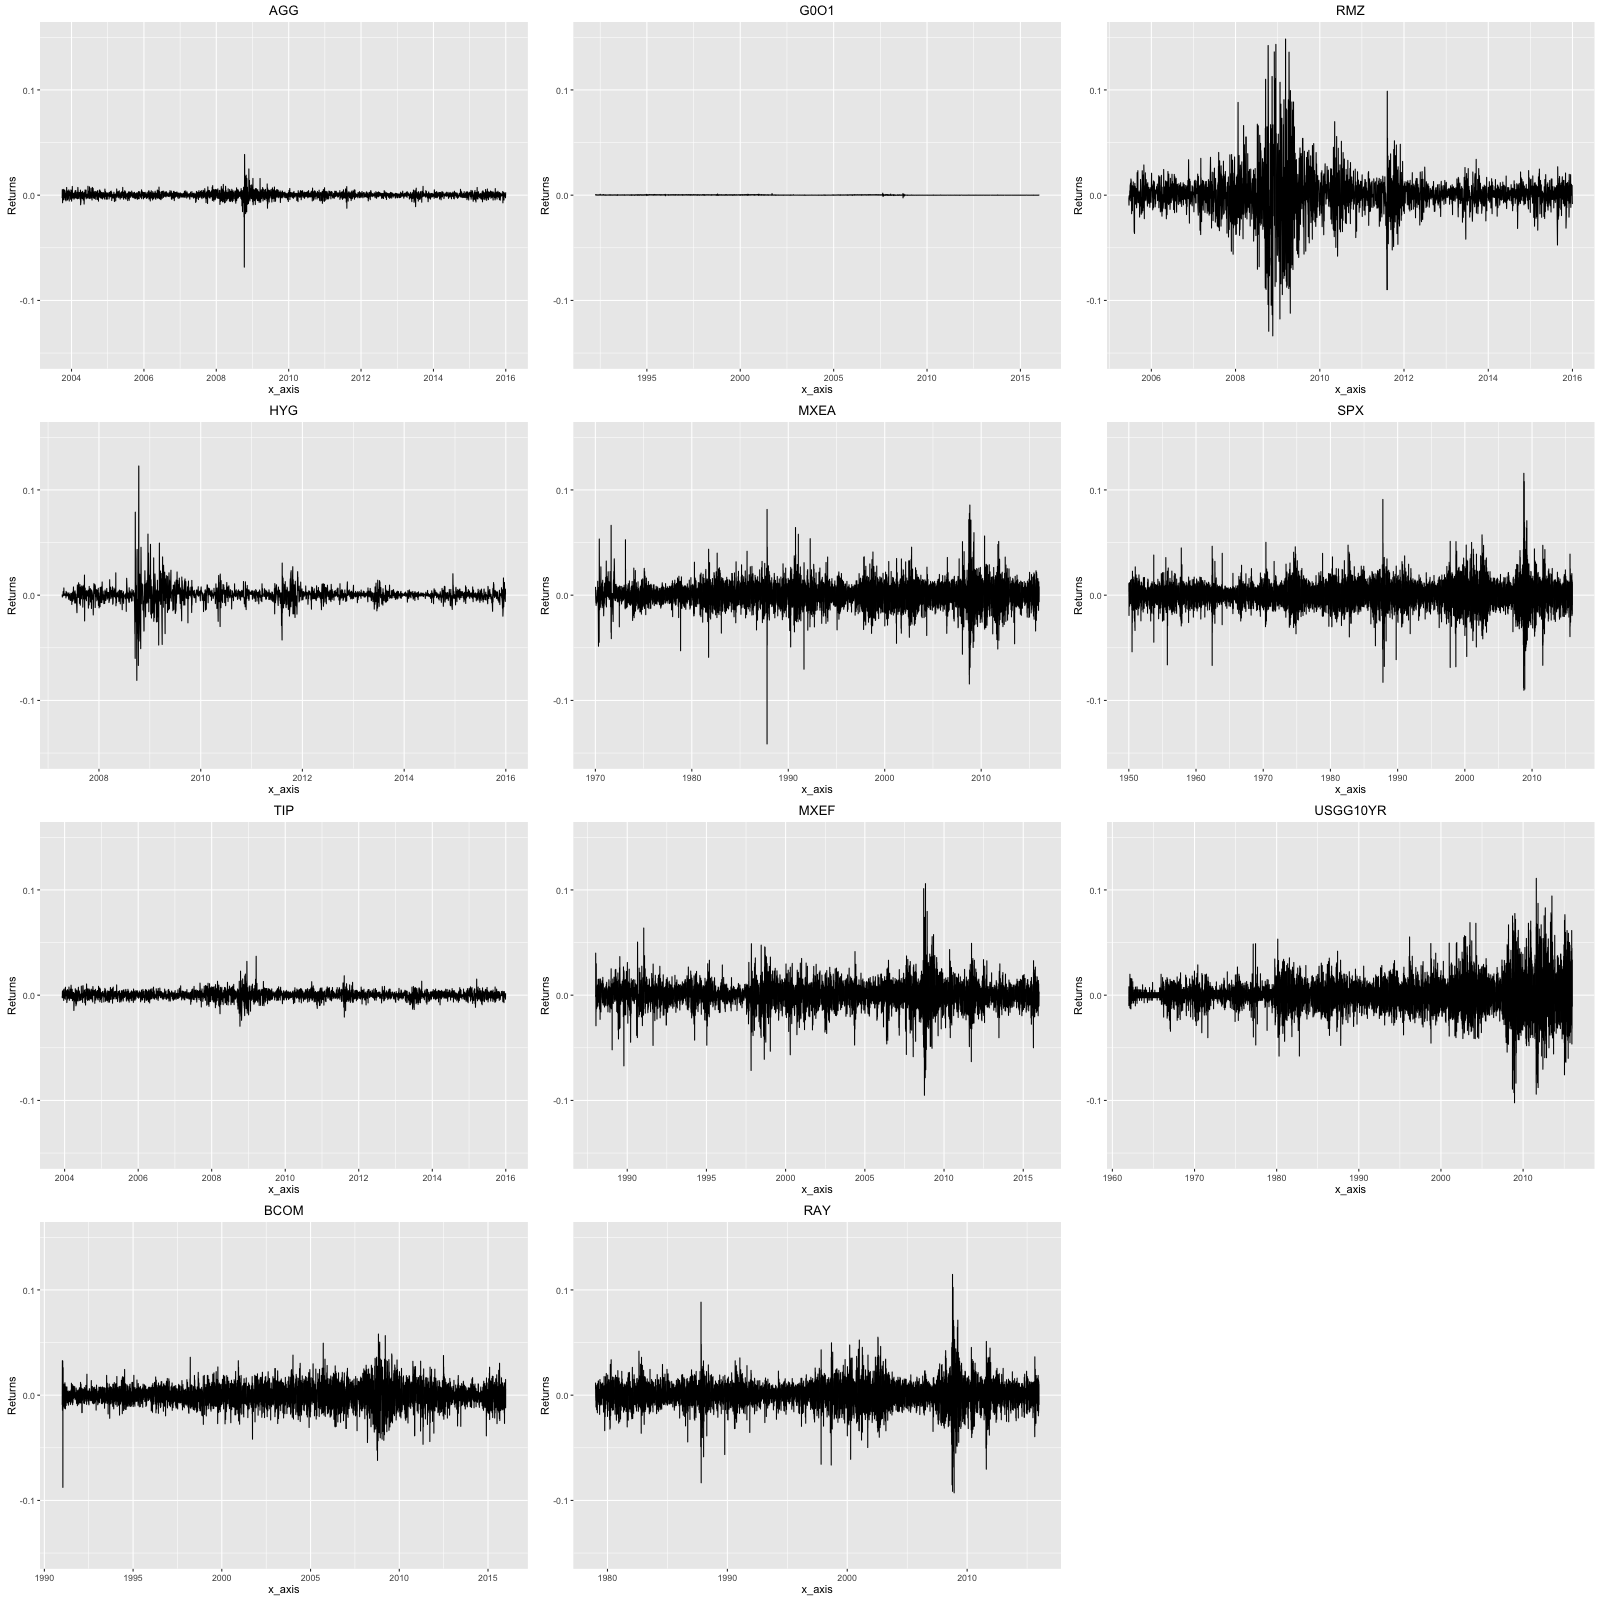
\includegraphics[width=15cm]{../results/returns}
\label{fig: dailyReturns}
\end{figure}

\begin{figure}[h]
\caption{Empirical distribution of daily returns} 
\centering 
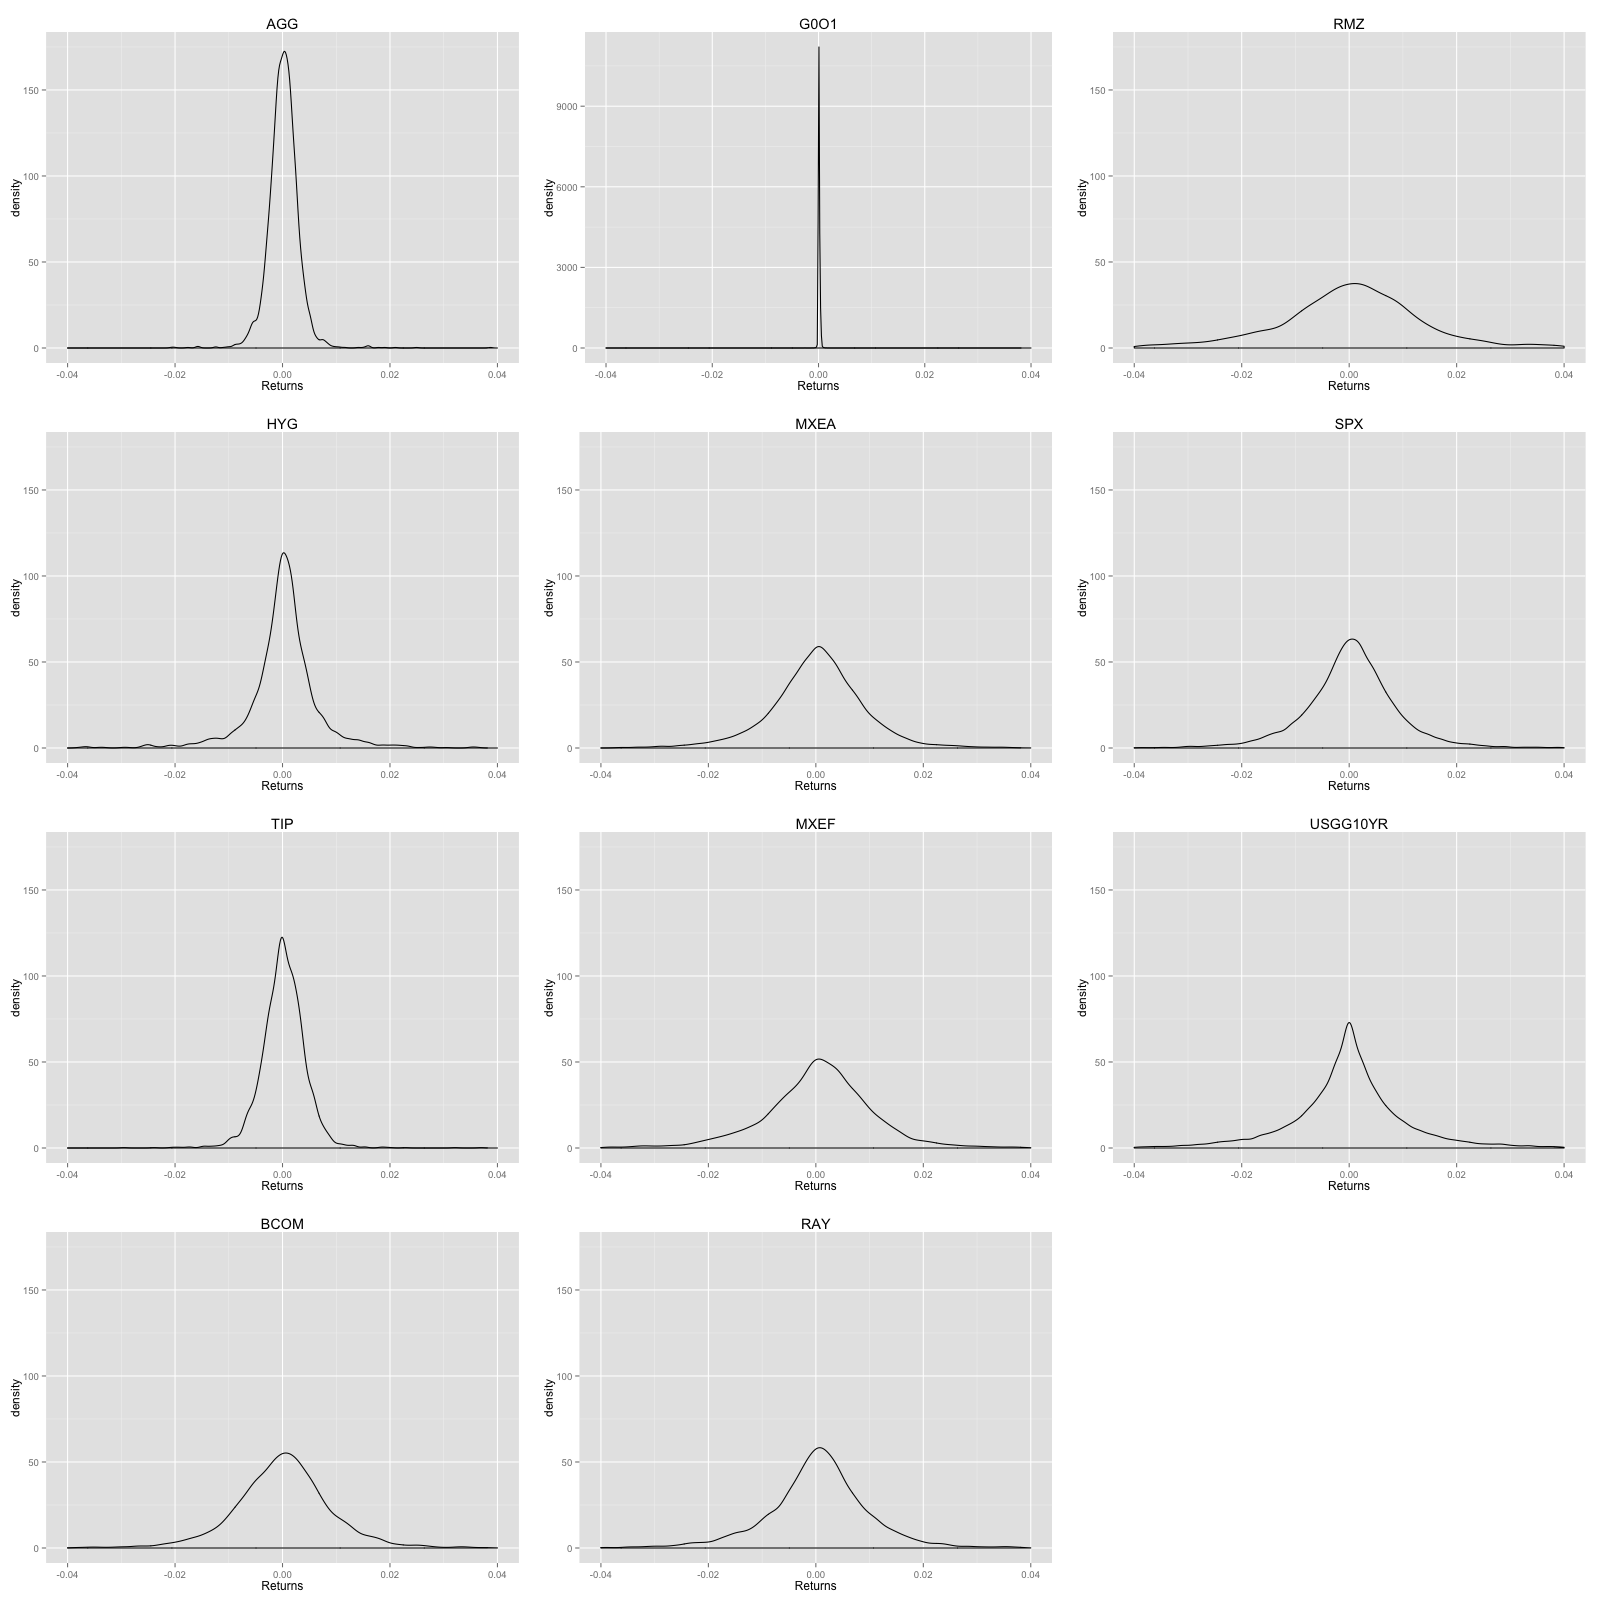
\includegraphics[width=15cm]{../results/returns_dist}
\label{fig: returnsDist}
\end{figure}

\begin{figure}[h]
\caption{Volatility under 6-month rolling window} 
\centering 
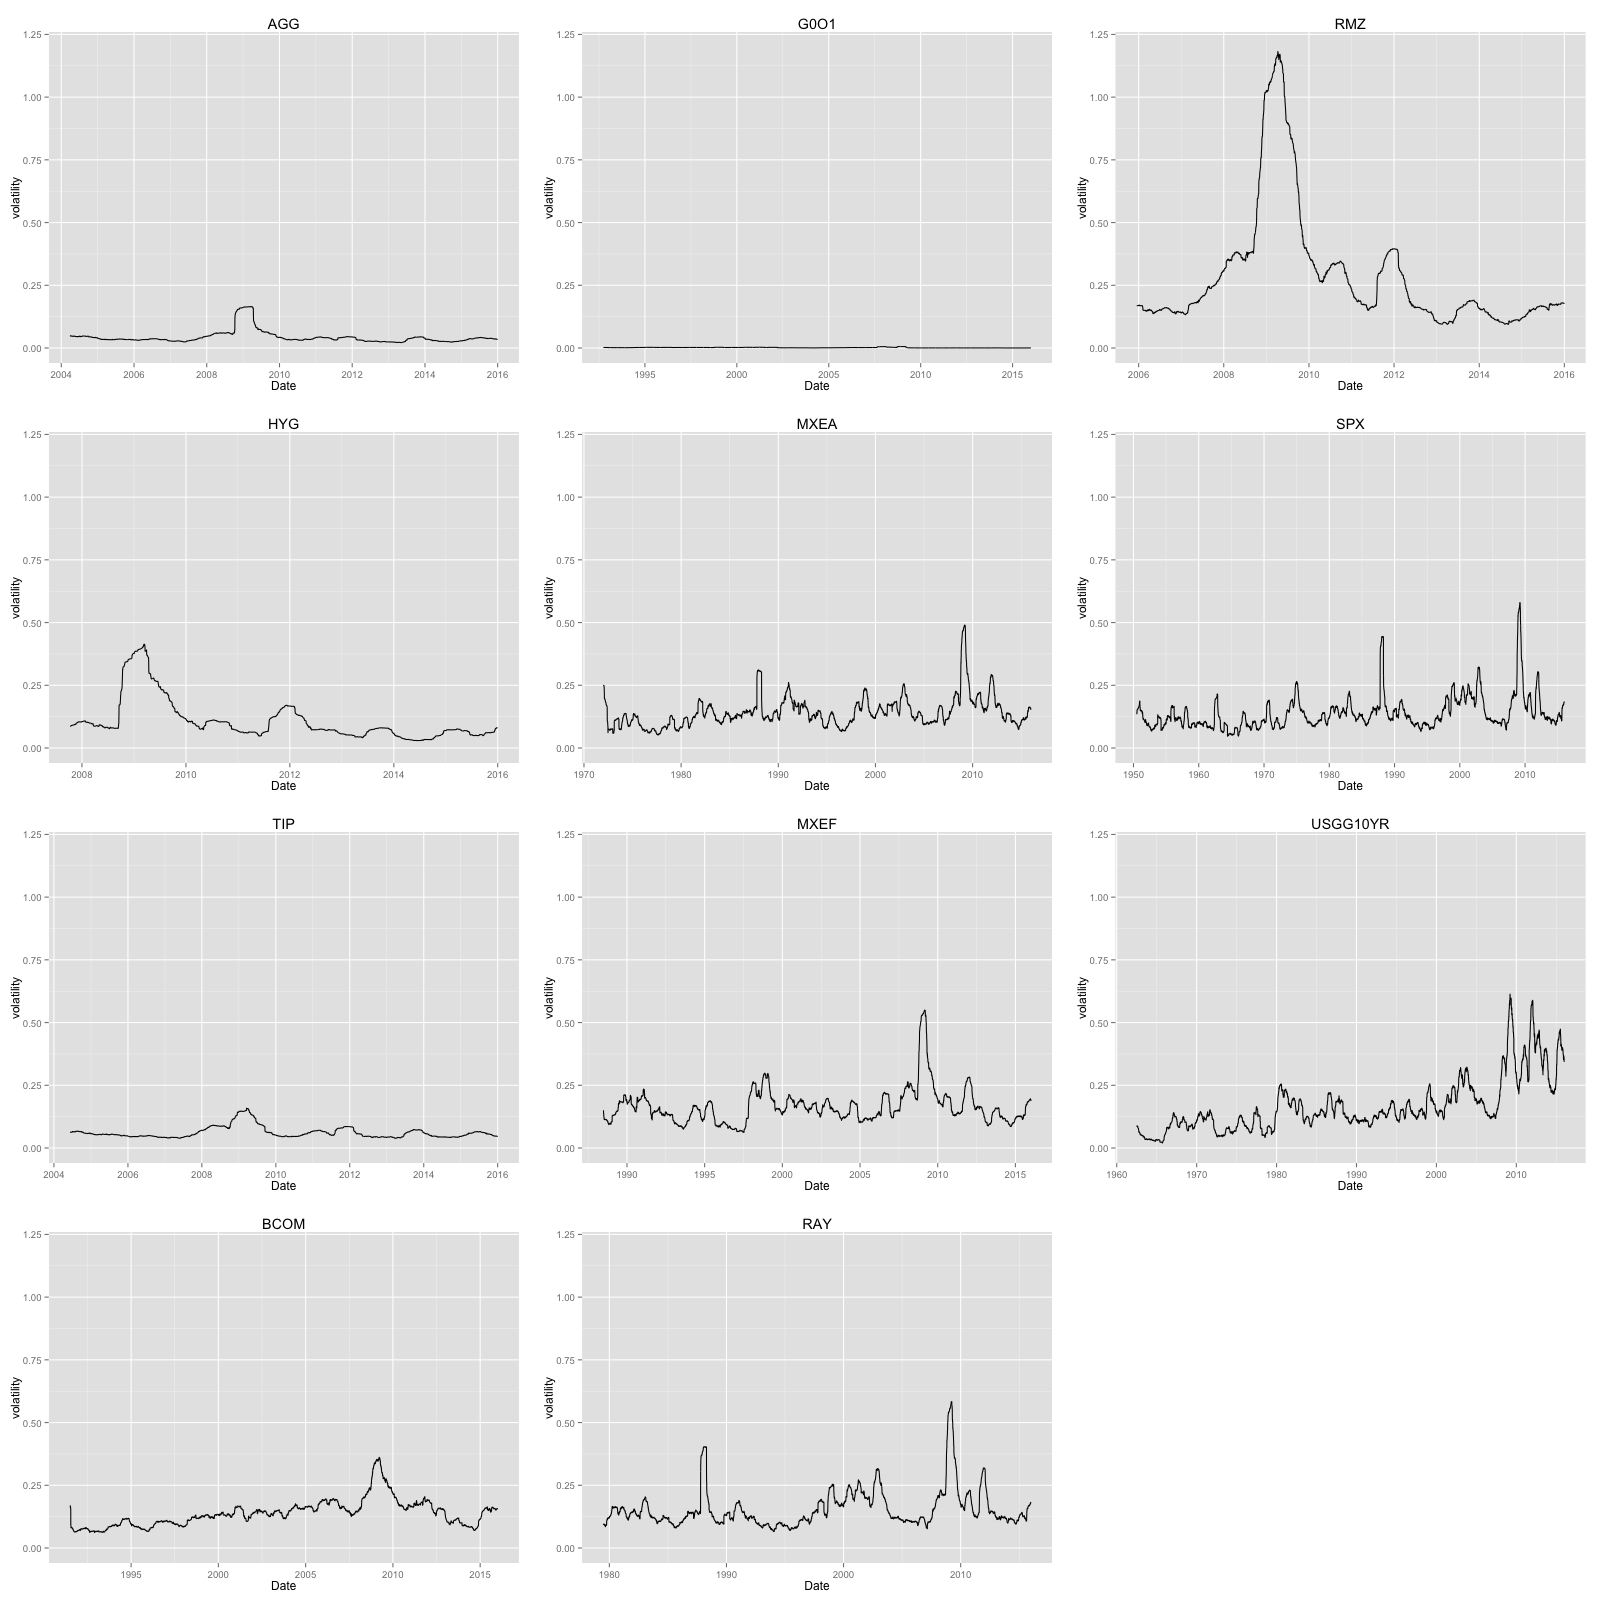
\includegraphics[width=15cm]{../results/volatility6mon}
\label{fig: variance6mon}
\end{figure}

\begin{figure}[h]
\caption{VaR(\%) under 6-month rolling window}
\centering 
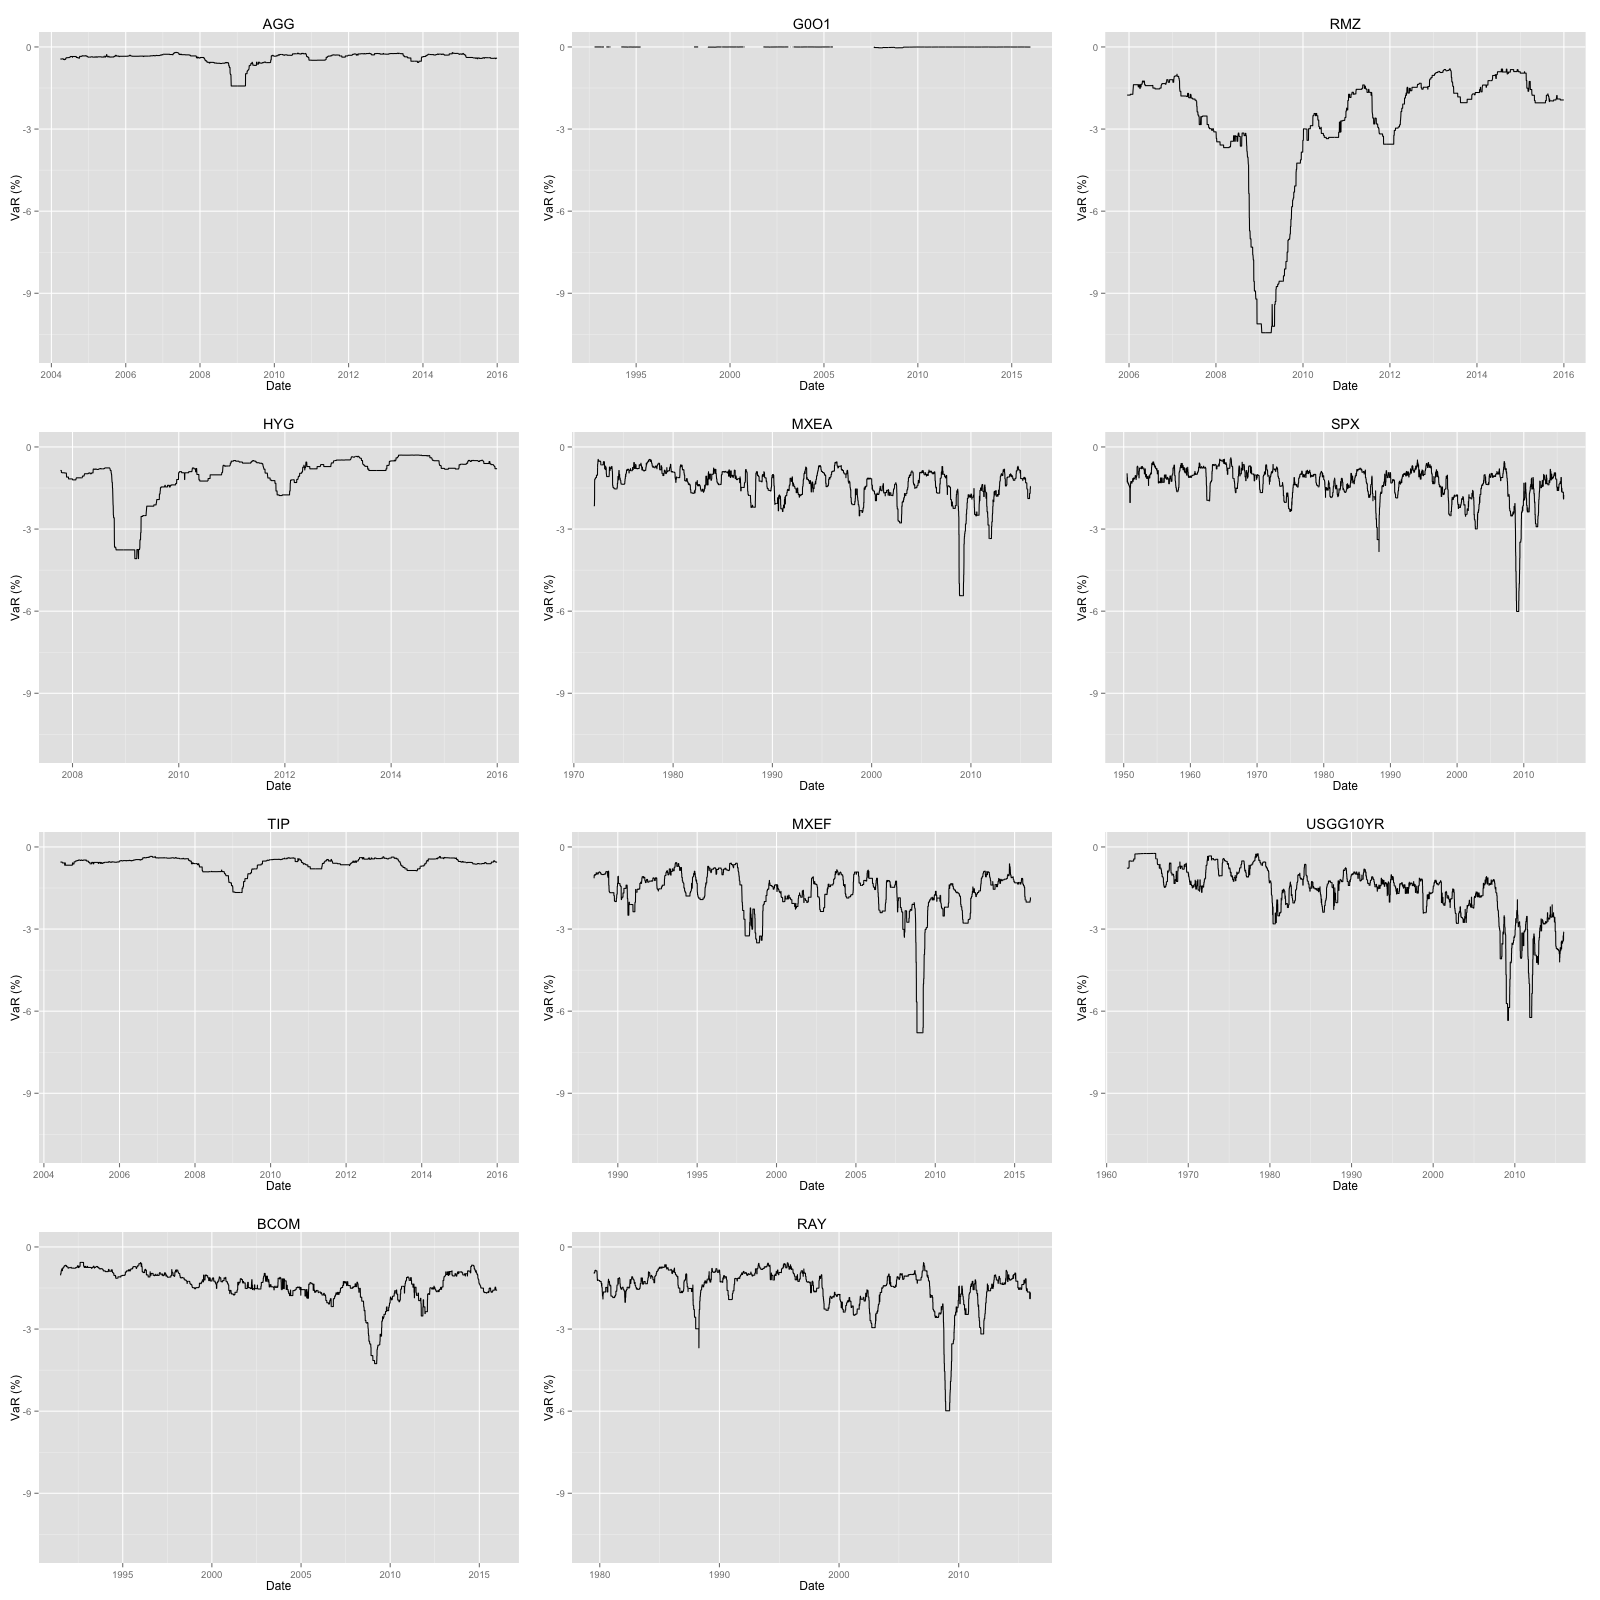
\includegraphics[width=15cm]{../results/VaR6mon_scaled}
\label{fig: VaR6mon}
\end{figure}

\begin{figure}[h]
\caption{ES(\%) under 6-month rolling window} 
\centering 
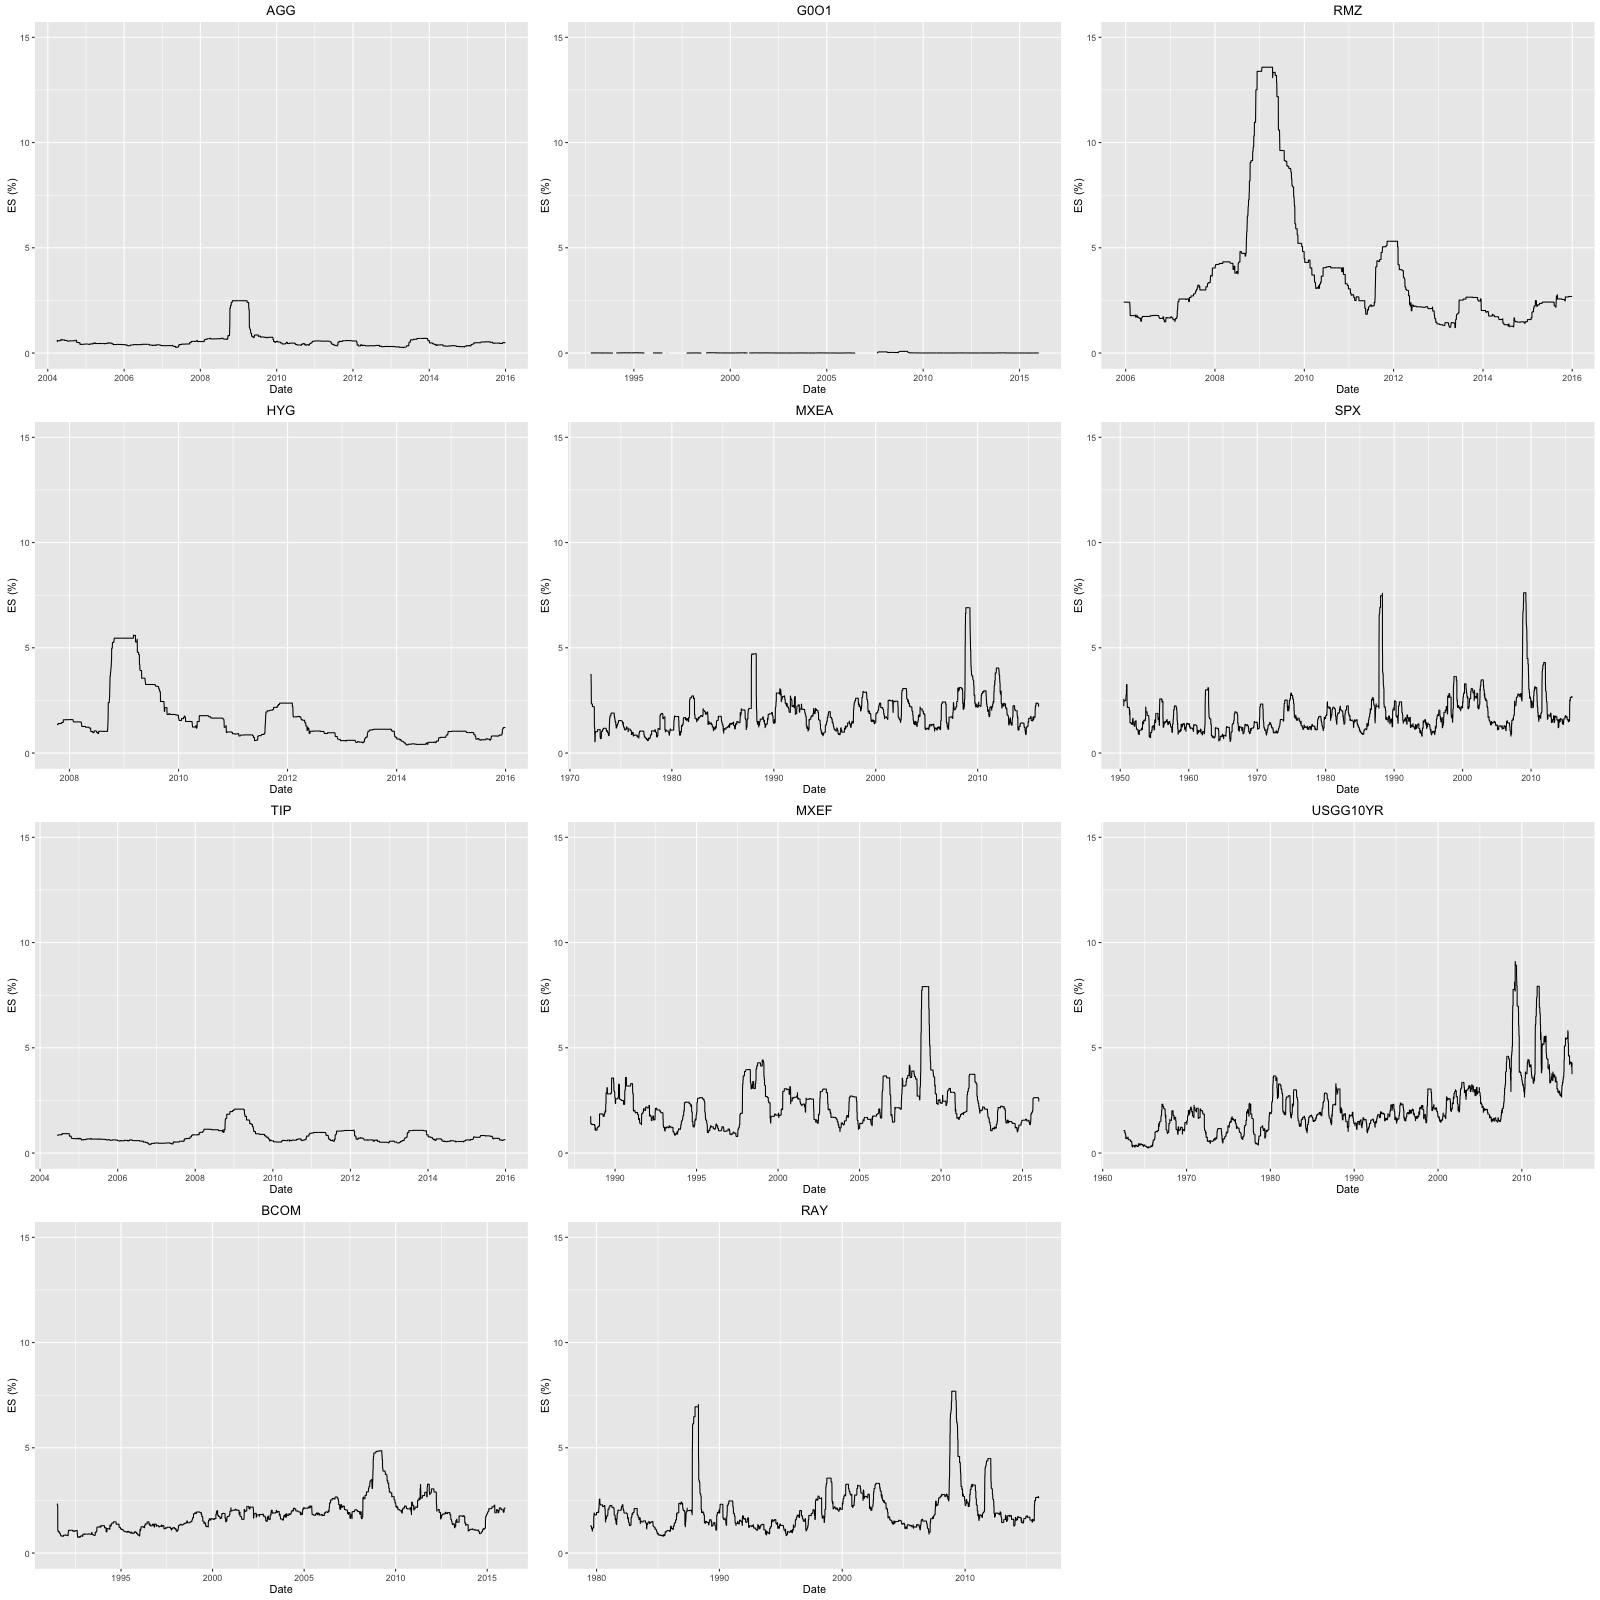
\includegraphics[width=15cm]{../results/ES6mon_scaled}
\label{fig: ES6mon}
\end{figure}



% \bibliographystyle{unsrt}
% \bibliography{analysis}

\end{document}
